\documentclass[aps,onecolumn,preprintnumbers,amsmath,amssymb,nofootinbib,superscriptaddress,notitlepage]{revtex4-1}

\usepackage{epsfig}
\usepackage[utf8]{inputenc}
\usepackage[dvipsnames]{xcolor}
\usepackage[normalem]{ulem}
%\usepackage{slashed}
\usepackage{caption}
\usepackage{amssymb}
\usepackage{mathtools}
\usepackage{bbold}
\usepackage{amssymb,latexsym}
\usepackage{amsmath,amsbsy,bbm}

\newcommand{\reales}{{\rm R}\hspace{-1ex}\rule{0.1mm}{1.5ex}\hspace{1ex}}
\def\tstrut{\vrule height2.5ex depth0pt width0pt} % used in tables
\def\jtstrut{\vrule height5ex depth0pt width0pt} % used in tables


\newcommand{\eftnopi}{\mbox{EFT$(\not \! \pi)$}}

\definecolor{green}{HTML}{2E8B57}
\interfootnotelinepenalty=10000 %% Completely prevent breaking of footnote

\begin{document}


%\title{Universally emergent L=1 resonances}
\title{Four-body L=1 systems from contact EFT}

\author{Johannes Kirscher}
\address{Theoretical Physics Division, School of Physics and Astronomy,\\
  The University of Manchester, Manchester, M13 9PL, UK}
  
\author{Martin Sch{\"a}fer}
\address{Nuclear Physics Institute of the Czech Academy of Sciences, 25069 \v{R}e\v{z}, Czech Republic}
  
\author{Rimantas Lazauskas}
\address{IPHC, IN2P3-CNRS/Universit\'e de Strasbourg BP 28, F-67037 Strasbourg Cedex 2, France}

\author{Lorenzo Contessi}\email{lorenzo@contessi.net}
\address{IRFU, CEA, Universit\'e Paris-Saclay, 91191 Gif-sur-Yvette, France}

\author{Jaume Carbonel}
\address{Universit\'e Paris-Saclay, CNRS/IN2P3, IJCLab, 91405 Orsay, France} 

\date{\today}




\begin{abstract} 
(to be cleaned at the end)
Few-body scattering resonances appear in multiple physical fields and are commonly found in experiments. 
Compared with boundstates, they are more difficult to be studied theoretically and numerically because of their belonging to the continuum phase-space.
In this study, we analyze the minimal theory that predicts the appearance of $L=1$ four-body resonance.
This state is known in nuclear physics to be related to the lighter nucleus that shows resonant behavior: $^4$H.
However, we aim not only to study it in the nuclear framework but also in more general universal systems.
For this purpose, we employ a contact effective field theory both fitted on nuclear observables (pionless effective field theory) and to unitary systems (universal effective field theory).
This study will help to understand how resonances emerge in few- and many-body systems for nuclear physics and any other physical field close to universality.
\end{abstract}



\maketitle

\section{Introduction}

Resonances are ever-present in quantum and classical physics.
However, especially in many-particle quantum fields as hadronic, nuclear, and atomic physics, they are far from been trivial to be predicted and calculated. 
A resonance in these fields is generally a consequence of a nonperturbative and complex interplay of particle-particle interactions and open channels that leads to the existence of multiple excitation and thresholds. 
The broad size and many-body nature make these states also relatively hard to be identified experimentally. 
Although many models predict the existence of resonant states with better or worse success, just looking at the Hamiltonian of a system it is hard to foresee their existence, and the numerical methods that can extract complex energy are, in general, expensive or less accurate than the ones developed for bound states.
%

%
Among nuclear systems with resonances, $^4$H $J^\pi=1^-$ has a special role and has been object of several studies as it is known to be the smallest nucleus with a (relatively broad) resonance.
%
In particular, cross-sections and scattering parameters have been studied extensively experimentally (e.g. \cite{osti_4230875, Phillips:1980zz, Tilley:1992zz}) and theoretically.
Concerning the theoretical side, several interactions and different numerical methods have been tested
(see, e.g. \cite{Ciesielski:1997vy,Ciesielski:1998sy,Ciesielski:1999pp,Viviani:1998gr,Fonseca:1999zz,Lazauskas:2004uq}) to predict well phaseshifts especially for low-energy scattering.
%
Fewer studies can be found, instead, about the position of the $^4$H resonance pole that induces such phaseshift. 
In \cite{Arai:2003ek,deDiego:2007rd,Lazauskas:2019cxj} the resonance position of $^4$H is extracted using respectively, RGM (which will be explained in the next sections of this paper), two-body $n-t$ potential, and three microscopic potentials with a Faddeev-Yakubovsky solver. 
The theoretical models agree for the presence of a $J^\pi=1^-$ resonance pole with energy $Re(E)=\{0.90 - 1.23\}$ MeV and width $\Gamma=\{3.5 - 5.8\}$ MeV.
Experimentally, the resonant pole can be extracted by R-matrix analysis to be at $Re(E)=3.50$ MeV and  $\Gamma=6.73$ MeV \cite{Tilley:1992zz}.
Although there is no precise agreement among experiment and models on the energy position of this resonant pole, the ability to create it in such models is still remarkable and has intrinsic value in the interpretation of the experimental cross-section.
%
The importance of studying $^4$H resonances and of the theoretical mechanisms that create it exceed the description of the system itself. 
It is the getaway for larger systems: on one hand for many-neutrons, on the direction of studying the stability of neutron tears and eventually to the neutron star equation of state.
On the other hand, to the study of resonances in heavy nuclei that are nowadays still hard or even impossible from ab-initio principles. 
%
In this study, we are interested in both these aspects on the framework of very minimalists nuclear forces: renormalizable contact effective field theories. 
%

%
In the last years, effective field theories (EFT) have had an ever-increasing impact on nuclear and atomic physics. 
They rely on the expansion of the appropriate underline theory onto a set of operators hierarchically arranged in a powercounting. 
The origin of this expansion depends on the kind of system in study and of the interparticle typical momentum exchanged, and differentiate an EFT from another. 
For example, it was shown that few-body nuclear systems are close to the unitary limit, in which the two-body scattering length is much larger than any other scale in such systems, allowing the description of few nucleons expanding the EFT around an infinite (or large) scattering length (see \cite{vanKolck:1999mw}).
This takes the name of pionless powercounting (\eftnopi) and, contrary to the chiral EFT, in which pions origin long-range forces, it is an expansion in contact operators.
The absence of pions in \eftnopi limits this theory to be a low-momentum theory (i.e. can not describe phenomena which typical momentum would allow the creation of pions) but allows it to be fully renormalizable and relatively easy to be treated numerically and analytically.
This makes it best suited to understand in simple terms even complex many-body phenomena and for the description of very shallow quantum states, like resonant poles. 
In the last years, \eftnopi was proven to be a valuable theory to study the behavior of many-boson systems and nuclei up to four nucleons. 
However, the LO of the theory does not appear to perform as well for the behavior of multi-fermionic systems, on which it erroneously predicts unbound nuclei above four particles (eg. $^7$Li and $^{16}$O) \cite{Schafer:2020ivj,Contessi:2017rww}.
The reason for this is to be attributed to the theory's more general inability of creating bound mixed symmetry states.
However, the subleading order of the EFT may still be able to correct this behavior provided that the LO creates, at least, an unbound state (virtual o resonant) that can be moved to the correct bound position. 
On the contrary, if no state is present at LO in these systems, of which $^4$H is the minimal representative, only a modification of the powercounting, and therefore of the entire theory, will allow for the correct description of nuclear physics using contact EFTs.
The creation of resonant poles in LO \eftnopi is possible, as it was shown in $nn\Lambda$ systems \cite{Schafer:2020rba} (as a subthreshold resonance), however, there is no record of such poles created in systems with mixed symmetry groundstates as $^4$H. 
By approaching the existence of a resonant pole in $^4$H we are tackling two problems at the same time: the possibility of creating resonances with the barest possible interaction and the fact that contact EFT can or not describe nuclear physics.
%


%
To access this state we first fix a \eftnopi on nuclear observables (fixing the nucleon mass, and the deuterium and triton bindings).
The same theory was also fixed to nuclear systems in which the two-body potential was tuned to the unitary limit.
This last case allows access to the universal limit and the deviation of the nuclear potential from it.
We chose to use a SU(4) symmetric theory in both cases for simplicity as this was proven to be a good first-order representation of nuclear physics \cite{Konig:2016utl}. 









\section{Contact EFT and numerical methods}

\begin{table}
    \centering
    \begin{tabular}{|ccc|}
    \hline
    \multicolumn{3}{|c|}{Nuclear LECs}\\
    \hline
         $\Lambda$ [fm$^{-1}$] & $C_0$ [MeV] & $D_0$ [MeV] \\
1   &	-44.4552	&	27.2312 \\
2	&   -142.376	&	172.703 \\
3	&   -295.959	&	559.013 \\
4	&   -505.202	&	1397.56 \\
6	&   -1090.66	&	6311.30 \\
10	&   -2929.48	&	89436.2 \\
    \hline
    \end{tabular}
    \quad
\begin{tabular}{|ccc|}
    \hline
    \multicolumn{3}{|c|}{Universal LECs}\\
    \hline        
        $\Lambda$  & $C_0$  & $D_0$  \\
1	&   -0.671	&	0.678 \\
2	&   -2.684	&	7.749 \\
4	&   -10.736	&	194.253 \\
6	&   -24.156	&	4273.294 \\
8	&   -42.944	&	122391.358 \\
10	&   -67.100	&	4102409.239 \\
    \hline
\end{tabular}
    \caption{LECs fitted for each cut-off. In the left tab are listed the LECs fitted to reproduce deuterium and $^3$He energy in MeV. On the right the ones that reproduce unitary systems of nuclei.}
    \label{tab:LECs_unprojected}
\end{table}


The leading order (LO) of the contact EFT we are employing consists of a contact two-body and a contact three-body operators with two low energy constants (LECs) to be fitted on physical observables \cite{vanKolck:1999mw}. 
A Gaussian regulator and a cut-off $\Lambda$ are introduced to smear the potential such that the contact limit is restored for $\Lambda\rightarrow+\infty$: 

\begin{equation}
    V(\textbf{r})=C_0 \sum_{i,j}^N e^{-\frac{r_{ij}^2\Lambda^2}{4}}
\end{equation}

\begin{equation}
    W(\textbf{r})=D_0 \sum_{ijk}^N \left[
    e^{-\frac{(r_{ij}^2+r_{ik}^2)\Lambda^2}{4}}+
    e^{-\frac{(r_{ij}^2+r_{jk}^2)\Lambda^2}{4}}+
    e^{-\frac{(r_{jk}^2+r_{ik}^2)\Lambda^2}{4}}\right].
\end{equation}

Once the interaction is regularized the LECs ($C_0$ and $D_0$) become cut-off dependent and must be fitted for any $\Lambda$ to reproduce the chosen set of fixed two- and three-body observables.
Nonetheless, if the theory is renormalizable this is sufficient to stabilize (in the sense of converging to a finite value) any other few- and many-body observable in the \textit{large cut-off limit}.
We employ two different two-body potentials in this study, a central one and one projected in S-wave only. 
This division is necessary for the numerical methods we use but is relevant only for small cut-offs.
In fact, in the limit, $\Lambda\rightarrow\infty$, the projected and unprojected potentials converge to the same contact interaction essentially representing only a different choice of the regulator.
Nonetheless, for small cut-off we expect and experience discrepancies, this results especially in different sets of three-body LEC $D_0$ that fix the three-body energy.
Moreover, for each projected and unprojected interaction we fit two sets of LECs.
The first, the "nuclear" one, fixes a single two-body boundstate of $B_2=2.22$ MeV (both in singlet and triplet channels).
In the second, the "universal" ones, the LECs are fitted to reproduce a large two-body scattering length ($a_0>10^5$).
In both cases, the three-body is fitted to reproduce a single three-body boundstate $B_3=-8.482$ MeV, and we employ the same nucleon mass to $m=938.858$ MeV, and the same $\hbar c= 197.31613$.
As an example, in tab. \ref{tab:LECs_unprojected}, we report the nuclear and universal LECs for the unprojected interaction.
%

%
Since \eftnopi is best suited for the description of low energy observables we refer to the effective range expansion (ERE) scattering parameter. 
It is essentially the expansion in low momentum of the phaseshift of a relative angular momentum $L$ two-body problem phaseshift $\delta$:

\begin{equation}
    k^{2L+1}cot(\delta)=-\frac{1}{a_L}+\frac{1}{2}r_L k^2 + ... \, .
\end{equation}

The same expansion can be used either in the two-body problem and in the four-body one assuming that $^4$H can be seen as a $n-^3$H pair.
Resonances will therefore emerge as poles of the system T-matrix

\begin{equation}
T = \frac{1}{k^{2L+1}cot(\delta)-ik}    
\end{equation}

and can be extracted either by fitting phaseshifts to the ERE formula or directly through solving the Schr\"odinger equation for complex energies. 




\subsection*{Numerical methods}

In this work, we utilize three different methods to solve the $n-^3$H shr\"oedinger equation.
The Rimas Method, the Stochastic Variational Method, and the Resonating Group Method. 
Coupled with these technologies we use also the complex rotation and the Analytic Continuation of the Coupling Constant (ACCC) to determine the position of resonant solution of the four-body problem (belonging to the continuum and hard to be extracted with the conventional methods) and the scattering lengths and volumes of the $n-^3H$ reaction. 

**wrong and to be changed** 
SVM consists of the variational search of the ground state of the problem using an over-complete set of Gaussians, chosen stochastically for each Jacobi coordinate, to represent the system wave function. 
This few-body method was developed by Lee Suzuki [] in ... and refined during the years to provide a reliable and relatively cheap solver for ground-state system up to $\sim 6$ particles.
A review of the method can be found in [] and a deeper insight is given by [].

%
%- Just give an idea and the references -
%
%
% RGM - SVM - ACCC - ?
%






%
%
%
%
%
%
%
%
%
%


\section{Procedure and results}

\begin{figure}
\centering
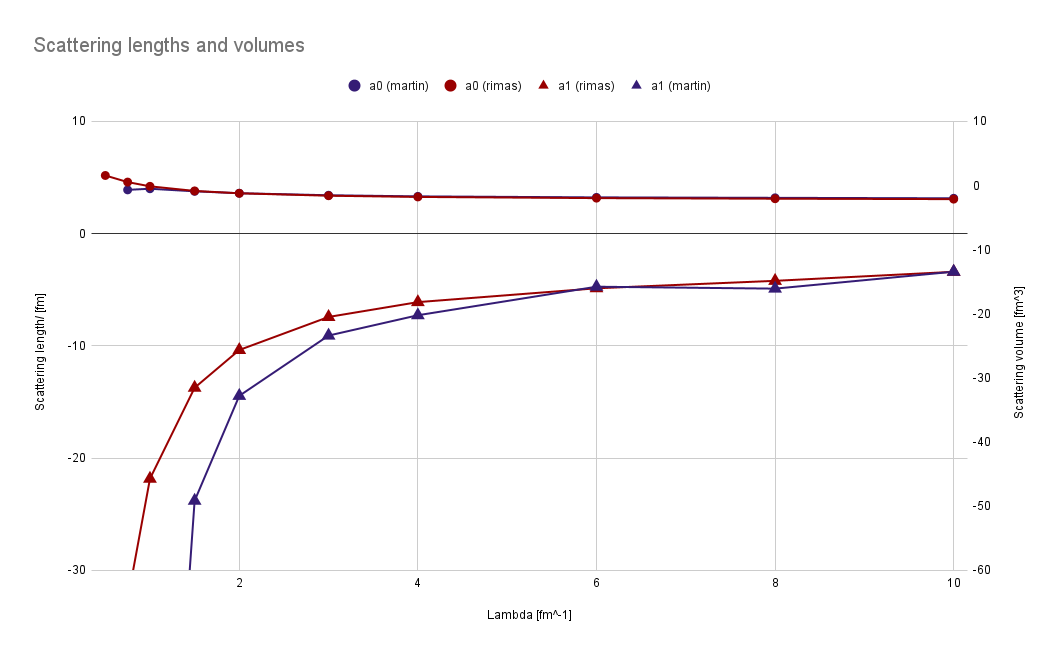
\includegraphics[width=0.95\textwidth]{./Graphs/a0a1} 
\caption{$1^-$ resonant pole in $^4$H}
\label{fig:a0a1}
\end{figure}


Our discussion begins with the analysis of low energy scattering parameters of the $n-^3$H system. 
This system allows for several low-energy states with relative angular momentum $J=1$ between the fragments: $0^-$, $1^-$, and $2^-$; we focus exclusively on the natural parity state: $1^-$. 
We also study the state $0^+$, with relative angular momentum L=$0$. 
This state is Pauli excluded, therefore, we do not expect any resonant or bound state in this channel but we still consider it interesting to study the EFT behavior and as a benchmark among different methods.
In figure \ref{fig:a0a1} we shown the scattering length and volume (relative to $0^+$ and $1^-$ states) calculated using SVM and RIMAS microscopical approaches.
Can be noticed how, for large enough cutoffs, the two methods are compatible.
This was expected since the two calculations use effectively two different regulators due to the presence of an S-wave projected and unprojected two-body potential. 
The difference between the two is more noticeable in the $J^\pi=1^-$ channel as the effect of P-wave interactions is more evident.
The two scattering parameters converge with the cut-off to a finite value. 
This fact is nontrivial since the interparticle interaction converges to a contact potential for large cut-offs.
In fact, $n$ and $^3H$ contain an identical fermion which suppresses any positive parity interaction.
However, the contact nature of the potential allows only particles in relative S-wave to interact. 
The finiteness of $a_0$ and $a_1$ should, therefore, be explained by the mediation of the distinguishable fermions and by the few-body effects.
$a_0$ and $a_1$ converge, empirically, as $1/\lambda$. 
In other words, since the interplay of S-wave interactions can result in a finite interaction in P-wave among few-body clusters, the scattering length/volume remains finite even only including the theory LO.
As a consequence, their cut-off behavior is $\propto1/\Lambda$ as expected by LO observables.
The sign and magnitude of the converged results ($a_0\simeq 3.1$ fm and $a_1\simeq-13(1)$) indicate the absence of boundstates, but the $a_1$ magnitude might indicate the presence of a shallow pole in the $1^-$ system.
It is also interesting to notice that the effective range for $0^+$ and $1^-$ remains also finite ($r_0\simeq2$ fm and $r_1\simeq1$ fm respectively).
This is also expected since, despite the nucleon-nucleon interaction is of contact nature, the size of the fragments remains finite, allowing for an inter-fragment long-range effect.
%

While arguably the best method to extract phaseshifts and resonance positions, the microscopic approach becomes more and more complicated and unfeasible when the number of particles is increased. 
For this, we would like to tackle the same problem from a different perspective: using the RGM formalism.
RGM intrinsically contains an approximation in the form of a simplified few-body wave function of one of the fragments.
It is, however, easily extendable to larger systems.
In our case, RGM transform a four-body problem into a simplified two-fragment one at the price of 




%
%
\begin{figure}
\centering
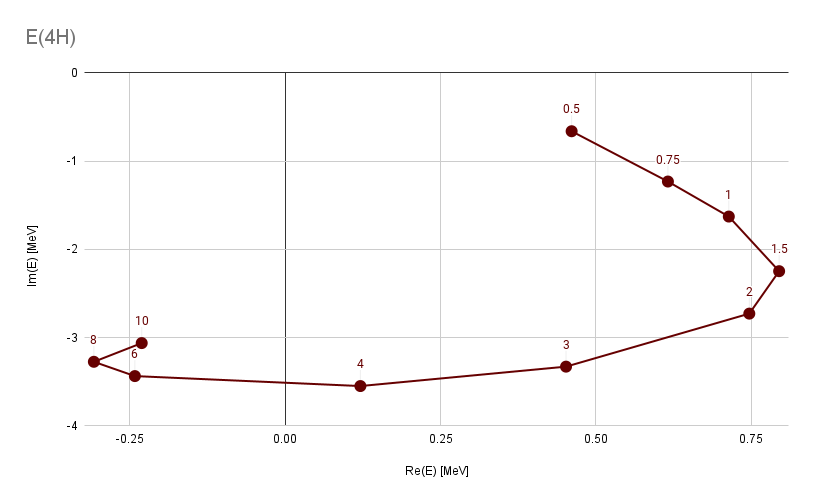
\includegraphics[width=0.95\textwidth]{./Graphs/E4H} 
\caption{$1^-$ resonant pole in $^4$H}
\label{fig:Resonance_pole}
\end{figure}
%

%
The second step in our calculation is the determination of the $J^\pi=1^-$ nuclear resonance position in the Energy complex plane. 
This has been done using the ACCC method starting from "RIMAS" numerical method. 
In figure \ref{fig:Resonance_pole}, the evolution of such pole can be follow to pass the threshold energy $B_{t}=8.484$ MeV ($Re(E)=0$ in the plot) to stabilize around $E_{n-t}=-8.7-i\,3.1$ for cutoffs greater than $6$ fm$^{-1}$.
This represents a shallow and broad subthreshold resonance. 
The presence of such a state and especially its stability (in this case expressed as a pole that does not run to infinite energy increasing the cut-off) is not trivial for the same reasons as one might not expect scattering length/volumes larger than zero.
%
Therefore, this proves that the theory is able to predict shallow states in systems with mixed symmetry. 
However, the position of the LO EFT pole appears to not be compatible with the physical resonance in $^4H$: ??? ($E_{n-t}=8.17+i\,6.73$). %\cite{http://tunlweb.tunl.duke.edu/nucldata/ourpubs/04_1992.pdf}. where does this come from? ???
Nonetheless, the theory is only tested at LO where the relevant operators to describe such states are not been yet introduced.
It is not in principle problematic that the LO pole is not consistent with the experimental data since including the subleading orders (NLO and N$^2$LO) can, even in a perturbative treatment of the expansion, relocate it in the correct position.
However, in this process one should be careful that the insertion of the subleading operators does not shift unreasonably, neither too much nor in the wrong direction, any of the other observables (e.g. the $^4He$ energy or the $n-^2H$ phaseshifts). 
At the current knowledge of the authors, no studies have ever been done in this sense and the possibility of a consistent correction of a resonant pole in therms of powerconting hierarchy remains to be demonstrated.
%




\subsection*{Universality}

%
In the framework of universal systems, in which the two-body scattering length is divergent, the scattering volume of $n-^3H$ follows an identical pattern as before, but with a convergent value of $\sim4$ fm$^3$.
This can be compared to the typical coordinate scale of the system, which, in this case, is uniquely identifiable with the three-body scale $R_3=(-2mE_3/\hbar^2)^{-1/2}\simeq 6$ fm. 
We find that $(a_1)^{-1/3}/R_3 \simeq  1/4$, which is a small, but still natural ratio.

** here I have some discrepancies (martin A11 is twice Rimas A11)
\begin{figure}
\centering
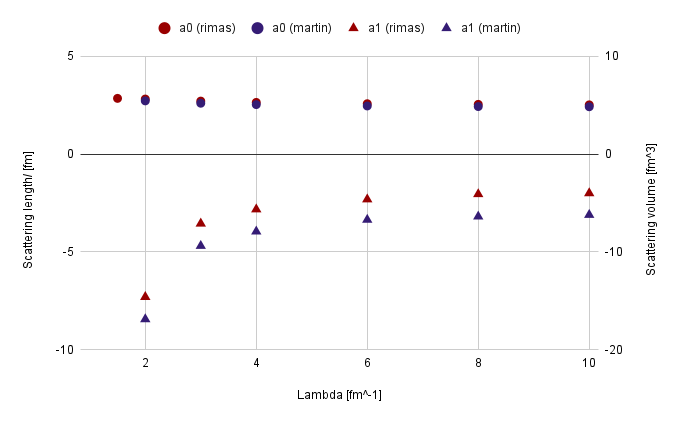
\includegraphics[width=0.95\textwidth]{./Graphs/unitarityA} 
\caption{Temporary: unitary scattering lengths / volume}
\label{fig:Resonance_pole}
\end{figure}
**[martin pole and data for unitarity]**






\section{conclusion}




\bibliographystyle{ieeetr}
%elsarticle-harv}
\bibliography{bibi.bib}

\section{Appendix: Resonating group method and interactions}
\end{document}